\section{Performing classical computations}

The quantum computer seems to have all the potential of performing computations that normal computers can't do, but it's not obvious that they can still perform the task of a normal one. That is a problem, in fact creating computers that are not able to perform simple tasks would be useless for us, and so we want to demonstrate that this isn't the case. 

The question "can quantum computers do classical computations?" comes from the doubt that in the possible operations that can be done on the qubits may not be able to simulate the two general operations that give rise to all the classical logic. These operations are the NAND gate and the COPY one, which together forms the building block of all the other possible operations. The first one is the \textbf{universal operation} of classical logic meaning that every circuit can be constructed using only NAND opeartions, while the latter constitute a problem due to some properties of QM that makes coping a non-trivial matter. Here we want to take the two properties one at a time and demonstrate that QC can perform both using the \textbf{Toffoli gate}.

\subsection{NAND operation}

The possibility of a QC to perform the NAND operation is not obvious, and the reason for that is the fact that all the quantum operations that we can perform on a qubit are invertible which the NAND is not. Basically it's not sure that a non-invertible operation can be constructed using invertible ones, or better if we can represent it using an invertible operation on a qubit. Fortunately turns out that performing the NAND on qubit is not only possible, but simple. The idea is using a Toffoli gate and setting one of the three qubits to $\ket{1}$, obtaining as output the NAND of the other two as we can see in the following circuit.

\begin{minipage}{0.4\textwidth}
    \centering
    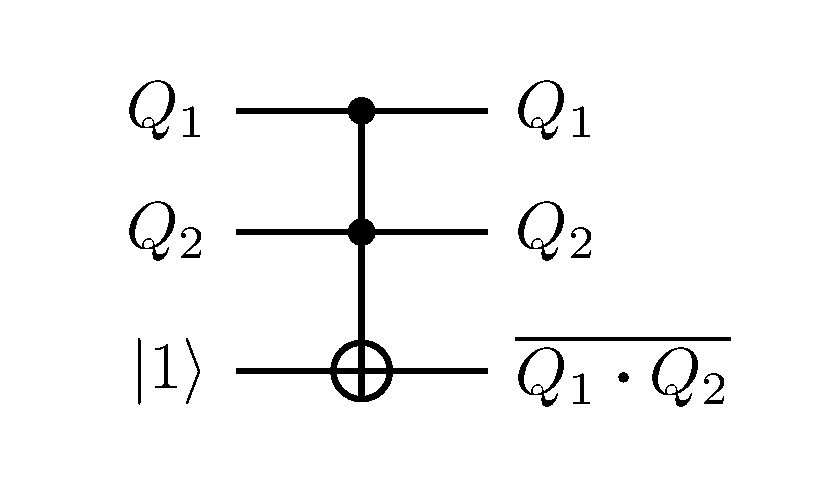
\includegraphics[width=\textwidth]{Immagini/NAND.pdf}
\end{minipage}
\begin{minipage}{0.45\textwidth}
    \centering
    \begin{tabular}{c|c}
        \textbf{IN} & \textbf{OUT}\\
        \midrule
        $\ket{001}$ & $\ket{001}$\\
        $\ket{011}$ & $\ket{011}$\\
        $\ket{101}$ & $\ket{101}$\\
        $\ket{111}$ & $\ket{110}$
    \end{tabular}
\end{minipage}

\noindent
Which clearly reconstruct the NAND as wanted, meaning that using QC we are able to recreate every possible classical circuit.

\subsection{Coping information}

First, we shall clarify why this operation represent a problem inside quantum circuits, and the reason is intrinsic inside QM and in the known result called \textbf{non-cloning theorem}, which states the following.
\thm{Non-cloning}
{
    Taken a state $\ket{\psi}$ of a system of qubit, it does not exist a unitary operation $\mathcal{U}$ with the following property
    \begin{equation}
        \label{eq:noCloning}
        \mathcal{U}\left( \ket{\psi}\otimes \ket{s} \right) = \ket{\psi}\otimes \ket{\psi},
    \end{equation}
    where $\ket{s}$ is another arbitrary state.
}
\pf{Proof}
{
    Let's imagine that such operation exist, and take three arbitrary states $\ket{\psi}$, $\ket{\phi}$ and $\ket{s}$. Since $\mathcal{U}$ is unitary the following relation must hold true
    \begin{equation}
        \braket{s\phi}{\psi s} = \braket{s}\braket{\phi}{\psi} = \mel{s\phi}{\mathcal{U}^\dagger \mathcal{U}}{\psi s},
    \end{equation}
    but using relation \eqref{eq:noCloning} and the normalization of the states it's possible to see that the latter equation becomes
    \begin{equation}
        \braket{\phi}{\psi} = \braket{\phi}{\psi}^2.
    \end{equation}
    This is not true in general, but only if we select carefully the two states in order for them to respect this relation. Otherwise, the operation $\mathcal{U}$ cannot be unitary and therefore is not a viable quantum gate.
}

This result may seem a problem by all means, but already in the proof is hidden the answer to overcome it. In fact, we have said that a cloning operation can exist if the starting states are selected carefully so that the norm of the states is conserved. In practice this means that we can use a Toffoli gate with two entries selected in a specific way to obtain the following copy gate.

\begin{minipage}{0.4\textwidth}
    \centering
    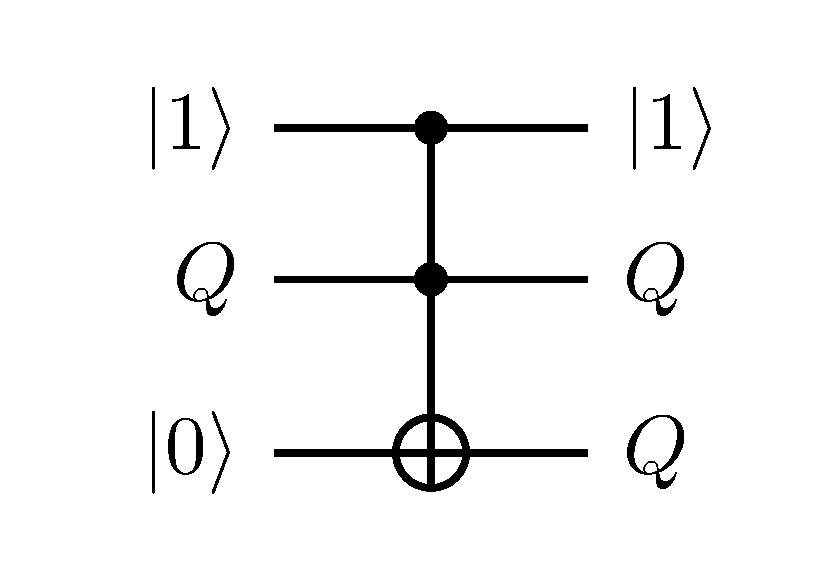
\includegraphics[width=\textwidth]{Immagini/Copy.pdf}
\end{minipage}
% \hspace{-1cm}
\begin{minipage}{0.45\textwidth}
    \centering
    \begin{tabular}{c|c}
        \textbf{IN} & \textbf{OUT}\\
        \midrule
        $\ket{100}$ & $\ket{000}$\\
        $\ket{110}$ & $\ket{111}$
    \end{tabular}
\end{minipage}

\noindent
In this way also coping information to one qubit to another can be done always using the Toffoli gate, making it probably the most important of all, and demonstrating that QC can perform all classical computations along with the unexplored quantum ones.